\section{Příklad 3}
% Jako parametr zadejte skupinu (A-H)
\tretiZadani{H}
\begin{figure}[H]
    \centering
    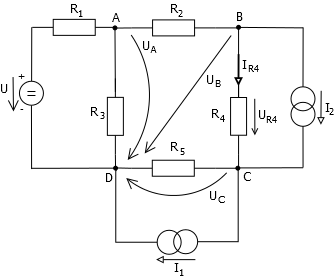
\includegraphics[scale=0.8]{pic3/Pr3_2022.png}
    \begin{quote}
        \centering
	   $\phi D = 0$ \\~\\
	   $I_{R1} - I_{R3} - I_{R2}  = 0$ \\
	   $I_{R2} - I_{R4} - I_2 = 0$ \\
	   $I_{R4} + I_2 - I_{R5} - I_1 = 0$ \\
    \end{quote}
\end{figure}
\newpage
\begin{quote}
    \centering
    $I_{R1} = \dfrac{(\phi D - \phi A + U)}{R_1} = \dfrac{U - \phi A}{R_1} $ \\~\\
    $I_{R2} = \dfrac{(\phi A - \phi B)}{R_2} $ \\~\\
    $I_{R3} = \dfrac{(\phi A - \phi D)}{R_3} = \dfrac{\phi A}{R_3}$ \\~\\
    $I_{R4} = \dfrac{(\phi B - \phi C)}{R_4} $ \\~\\
    $I_{R5} = \dfrac{(\phi C - \phi D )}{R_5} = \dfrac{\phi C}{R_5} $ \\~\\ 
\end{quote}
\begin{quote}
    \medskip
    \medskip
    \centering
    $\dfrac{U}{R_1} - \dfrac{\phi A}{R_1} -  \dfrac{\phi A}{R_3} - \dfrac{\phi A}{R_2} + \dfrac{\phi B}{R_2} = 0$ \\~\\ 
    $\dfrac{\phi A}{R_2} -  \dfrac{\phi B}{R_2} - \dfrac{\phi B}{R_4} + \dfrac{\phi C}{R_4} - I_2 = 0$ \\~\\ 
    $\dfrac{\phi B}{R_4} - \dfrac{\phi C}{R_4} + I_2 - \dfrac{\phi C}{R_5} - I_1 = 0$ \\~\\ 
\end{quote}
\begin{quote}
    \medskip
    \medskip
    \centering
    $-\phi A * (\dfrac{1}{R_1} +  \dfrac{1}{R_2} + \dfrac{1}{R_3}) + \phi B * (\dfrac{ 1}{R_2} )  = -\dfrac{U}{R_1}$ \\~\\ 
    $\phi A * (\dfrac{1}{R_2}) - \phi B * (\dfrac{1}{R_2} + \dfrac{1}{R_4} ) + \phi C * (\dfrac{1}{R_4})  = I_2 $ \\~\\
    $\phi B * (\dfrac{1}{R_4}) - \phi C * (\dfrac{1}{R_4} + \dfrac{1}{R_5})  = I_1 - I_2 $ \\~\\
\end{quote}
\begin{align*}
	\begin{pmatrix}
		-(\dfrac{1}{47}+\dfrac{1}{39}+\dfrac{1}{58})&\dfrac{1}{39}&0\\
		\dfrac{1}{39}&-(\dfrac{1}{39}+\dfrac{1}{28})&\dfrac{1}{28}\\
		0&\dfrac{1}{28}&-(\dfrac{1}{28}+\dfrac{1}{25})
	\end{pmatrix}\times
	\begin{pmatrix}
		\phi A\\
		\phi B\\
		\phi C
	\end{pmatrix}=
	\begin{pmatrix}
		-\dfrac{130}{47}\\
		0.5 \\
		0.45
	\end{pmatrix} \\
	\begin{pmatrix}
		\phi A\\
		\phi B\\
		\phi C
	\end{pmatrix}=
	\begin{pmatrix}
		-20,2480& -11,6646& -5,5022\\
		-11,6646& -29,1872& -13,7676\\
		-5,5022& -13,7676& -19,7017
	\end{pmatrix}\times
	\begin{pmatrix}
		-\dfrac{130}{47}\\
		0.5 \\
		0.45
	\end{pmatrix}
\end{align*}

\begin{quote}
    \centering
    $\phi A = 47.6969 \Vo$ \\ 
    $\phi B = 11.4748 \Vo$ \\
    $\phi C = -0.5307 \Vo$ \\ 
    \medskip
    \medskip
    $I_{R4} = \dfrac{(\phi B - \phi C)}{R_4} = \dfrac{( 11.4748\Vo + 0.5307 \Vo)}{28\Omega} = 0.4287\Am$ \\~\\
    $U_{R4} = \phi B - \phi C = 11.4748 \Vo + 0.5307 \Vo = 12.006\Vo$
\end{quote}
 